\documentclass[letterpaper,12pt]{article}

\RequirePackage{comment}
\RequirePackage[hypertex]{hyperref}
\RequirePackage{GE05}
% this inputs graphicx, too

\newcommand{\NX}{\mbox{\em NX\/}}
\newcommand{\POP}{\mbox{\em POP\/}}

\def\ClassName{The Global Economy}
\def\Category{Professor David Backus}
\def\HeadName{Midterm Examination}

\begin{document}
\parindent = 0.0in
\parskip = \bigskipamount
\thispagestyle{empty}%
\Head

\centerline{\large \bf \HeadName}%
%\centerline{March 9, 2005}
\centerline{Revised:  \today}

\bigskip
You have 75 minutes to complete this exam.  Please answer each
question in the space provided. You may consult one page of notes
and a calculator, but devices capable of wireless transmission are
prohibited.

I understand that the honor code applies: I will not lie, cheat,
or steal to gain an academic advantage, or tolerate those who do.

\begin{flushright}
\rule{4in}{0.5pt} \\ (Name and Signature)
\end{flushright}

\begin{figure}[h]
    \centering
    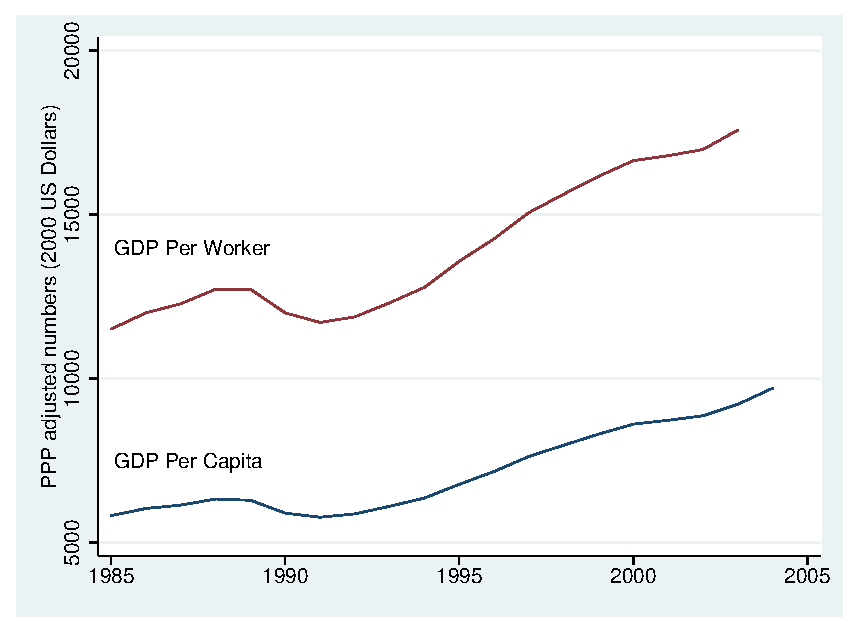
\includegraphics[scale=0.8]{pwtpolypopyl.eps}
    \caption{GDP Per Capita and GDP Per Worker in Poland.}
    \label{fig:poland}
\end{figure}

\begin{enumerate}
% ======================================================================
\item {\it Poland goes to market.\/} 
After four decades as a centrally-planned economy, 
Poland made what it termed a ``shock transition'' to a market system, 
in which prices were set by the market rather than the government.  
Between 1988 and 1992, GDP per capita fell, 
but since 1992 growth has been steady and dramatic.  
Your mission:  use the data in Table \ref{tab:poland} 
to quantify Poland's recent experience 
and speculate about its sources.   

%
\begin{table}
    \centering 
    \tabcolsep = 0.2in
    \begin{tabular}{lcccc}
    \hline\hline
    Year    &  $Y/\POP $  &  $Y/L$  &  $K/L$  & $K/Y$  \\
    \hline\hline
    1988 &  6,327 &  12,724  &  33,061  &  2.60 \\
    1992 &  5,875 &  11,882  &  32,622  &  2.75 \\
    2003 &  9,216 &  17,575  &  39,462  &  2.25 \\
    \hline\hline
    \end{tabular}
    \caption{Output, Capital, and Labor in Poland.
    Data from the Penn World Tables.  
    $\POP$ is population, $Y$ is GDP (output), 
    $L$ is employment, and $K$ is capital (plant and equipment).  
    $Y$ and $K$ are PPP-adjusted numbers, expressed in 2000 US dollars.}
    \label{tab:poland}    
\end{table}
%

\begin{enumerate}

\item During the transition period, 1988-92, 
what were the growth rates of GDP per capita 
and GDP per worker?  
What does their difference tell you? 
If markets are such a good idea, 
why didn't output increase immediately?  
(15~points)

\item During the market period, 1992-2003, 
what were the sources of growth in GDP per capita?  
Note specifically the roles of employment and 
total factor productivity.  
(20~points)

\item You would like to update the data, 
but the Penn World Tables end in 2003.  
You decide to look at the EIU's database, 
where you find data on population, employment, 
investment, and output, 
but not the capital stock.
Show how you can use the connection between capital 
and investment to update the former.  
To be specific, 
show how you can generate the 2004 value of $K/Y$
from real GDP growth (5\%), depreciation (6\%), 
the ratio of investment to GDP ($I/Y = 0.19$), 
and the 2003 value of $K/Y$.    
(5~points)
\end{enumerate}


%\begin{comment}
Answer.
\begin{enumerate}

\item We compute the usual continuously-compounded growth rates.
The growth rates were --1.85\% (GDP per capita)
and --1.71\% (GDP per worker). 
The modest difference between them reflects the difference 
in their denominators:  population v employment/workers. 
Since GDP per worker grew faster (less slowly), 
evidently the number of workers
grew more slowly than the population. 
Why didn't output grow?
One guess is that the transition takes time:  
even if you think the market orientation will improve
performance, it could take a few years.  

Grading:  10 points for computing the growth rates correctly
(partial credit for something along these lines), 
2 for understanding the source of the difference between them
(ie, $L/\POP$), 
and 3 for any reasonable comment about the transition.  

\item The usual growth accounting exercise.  
Our decomposition of the growth rate of output per worker is 
\begin{eqnarray*}
        \gamma_{Y/\POP} &=& \gamma_{L/POP} + \gamma_{Y/L} \\
            &=& \gamma_{L/POP} + \gamma_A + \alpha \gamma_{K/L}  .
\end{eqnarray*} 
with $\alpha = 1/3$.
The letter $A$ stands for total factor productivity (TFP).    
The numbers are 
\begin{eqnarray*}
     4.09 &=& 0.53 \mbox{ (L/POP)} + 2.98 \mbox{ (A)} 
                +  0.58 \mbox{ (K/L)} .
\end{eqnarray*}
As we often find, most of the action is in TFP ($\gamma_A$).  

Grading: 20 points for getting the numbers exactly right, 
partial credit for other answers.  
16 points for a correct decomposition of output per worker, 
rather than the requested output per capita.  

\item The idea is that we can ``bootstrap'' capital numbers using 
investment.  
Recall
\begin{eqnarray}
    K_{t+1} &=& (1-\delta) K_t + I_t .
    \label{eq:lom-k}
\end{eqnarray} 
Since the data are expressed as ratios to GDP, we would use
something like
\begin{eqnarray*}
    K_{t+1}/Y_{t+1} &=& 
        (Y_t/Y_{t+1}) \left[ (1-\delta) K_t/Y_t + I_t/Y_t \right] .
\end{eqnarray*} 


Grading: 3 points for mentioning equation (\ref{eq:lom-k}), 
1 for anything beyond that, 
1 more for the second equation.  

\end{enumerate}
%\end{comment}


%\pagebreak \phantom{xx} \pagebreak %\phantom{xx} \pagebreak
% ======================================================================
\item {\it Retail banking in Latin America.\/}
Your first day as a summer intern at Banco Santander, 
your supervisor asks you to give a brief report after lunch on 
the institutional factors that might guide Santander's
goal of expanding its retail businesses in Latin America:
consumer lending, small business lending, credit cards, and so on.  
Santander, as you know, is a major player in the region, 
and regards it as a potential growth opportunity. 
You immediately turn to the Global Economy resource page and collect
the information in Table \ref{tab:institutions}.

%
 \begin{table}
%    \tabcolsep = 0.2in
    \centering
    \begin{tabular}{lcccc}
    \hline\hline
    Indicator    &  Brazil   & Colombia  &  Peru  &  Venezuela \\
    \hline\hline
    GDP per capita (USD) &  10,300  &  9,000 &  8,500  & 14,000 \\
    Political stability  &  35 &  10  &  20  &  10 \\
    Rule of law          &  45 &  35  &  30  &  5  \\
    Control of corruption&  55 &  50  &  45  &  10 \\
    Contract enforcement &  84 &  48  &  64  &  56 \\
    Credit information   &  50 &  50  &  60  &  0 \\
    \hline\hline
    \end{tabular}
    \caption{Measures of performance and institutional quality.
        Higher numbers indicate better institutional quality.}
    \label{tab:institutions}
\end{table}
%
Based on this information and your own good judgment, 
what would you tell your new colleagues? 
Which countries do you think offer the most attractive opportunities?  
Why?  
What issues do you think deserve closer scrutiny?    
(30~points) 

%\begin{comment}
Answer.  This is a relatively unstructured question, 
so there's no single best answer.  
A good answer probably touches on the following points:
%
\begin{itemize}
\item GDP per capita. 
This is a rough estimate of how much income people have.
Here you see Venezuela is a bit above the others.  

\item General institutions. 
Things like political stability, rule of law, 
and control of corruption all reflect the quality of the 
economic environment.  
Here Brazil looks best, Venezuela worst.  

\item Specific institutions.  
These relate directly to lending and credit cars:  
contract enforcement and credit information 
(availability of databases used to credit credit scores).  
Again, Brazil looks pretty good.  

\item Bottom line.  Your call.
Brazil looks pretty good to me overall, 
with Peru a possible second.  
I'd want to collect more information about the last two:
How hard is it to collect a debt?  
What does the local credit industry look like?  
Are there competitors whose experience would be informative?  

\end{itemize}

Grading:  20 points for anything sensible, 
30 for an articulate well-reasoned argument that hits these points
or otherwise makes a persuasive argument with the information
given in the question. 

%\end{comment}


%\pagebreak \phantom{xx} \pagebreak %\phantom{xx} \pagebreak
% ======================================================================
\item {\it Miscellany.\/}
\begin{enumerate}

\item {\it Food prices.\/}
When food prices rose sharply in 2008, India restricted
food exports to keep prices down. 
Who would you expect to benefit from this policy?  Lose?  
Is the overall impact on the Indian economy likely to be 
positive or negative?   
(10~points)

\item {\it Layoffs.\/}
From the New York Times, March 6, 2009 (rough paraphrase):   
The WARN Act requires employers to give 60 days' notice 
if a plant is closed or 500 or more people are laid off at one location.  
Some wonder whether notice should be required for other job losses.
A Berkeley professor says  
it's a matter of ``transparency and decency.'' 
An IBM executive disagrees, noting that it's routine for the company to lay off some employees while hiring others.  
``This business is in a constant state of transformation.''  
If you were asked to advise President Obama, 
how would you describe the costs and benefits of 
wider application of the WARN Act?  
(10~points) 

\item {\it Inflation.\/} 
Government statisticians routinely adjust prices for changes 
in the quality of products.
PIMCO's Bill Gross thinks it's a scam:
``The government says that if the quality of a product goes up, 
then its price really didn't go up and may actually have gone down.  
Why does the US government continue to foist this on a gullible public when they should know better?  They do a disservice to those grounded in the reality of trying to stretch a paycheck.''
Do you agree with him?  Why or why not?  
(10~points)
\end{enumerate}


%\begin{comment}
\pagebreak 
Answers.  
\begin{enumerate}
%
\item You might expect this to keep prices down in the short run 
because we've reduced the demand for locally produced food.
(You could also express this as an increase in supply to the domestic market, but it's cleaner this way.) 
Who gains:  domestic food buyers, foreign producers.
Who loses:  domestic sellers/producers, foreign buyers.  
Generally, any market intervention like this is a net loss. 
You could show this formally using a supply and demand diagram.  

A related issue is that high prices might be expected to encourage 
an increase in production.
We missed out on that by keeping prices low.  
In fact, we would expect supply to fall, which makes things worse.  
Interesting to me but not part of the question:  
I would expect poor people to be among the producers, so it's not clear to me why this policy was so popular.   

Grading:  5 for any sensible argument, 
up to 10 for something better. 

\item  I'd guess that this is another cost of firing workers, 
and we know that higher firing costs tend to discourage firms
from hiring workers in the first place.  
The question is how high the cost is.  
If we figure workers will keep producing, it may be small, 
but I'd guess it was closer to adding 60 days to severance.  
And there's probably red tape associated with such a law.  

I asked to two of my favorite management professors 
the same question.
Professor Wiesenfeld said:  
``I think giving people advanced notice (not 60 days, but not escorting them to the door immediately) is generally beneficial, 
because it helps to retain the commitment and motivation of the person's former colleagues.''
Professor Freedman said:  
``It depends on the situation.  It has the potential to be extremely serious. For example, I have encountered situations where people who are given notice act in a very destructive manner.''
He adds:  
``In bad times the flexibility [to fire some people and hire others] 
is much more important than in good times because organizations have less slack.''

Grading:  5 for any sensible argument, 
up to 10 for something better. 
Better should include a discussion of whether this is a large 
cost or a small one.  

\item The idea is this.  Suppose in 2000 I buy a TV for \$250, 
and in 2005 a TV costs \$300.  That looks like inflation.
But suppose the 2005 TV is 50\% better:  then quality adjusted prices
have fallen from (say) 250 to 200 
(300 for the equivalent of 1.5 TVs).  
That's what the official numbers do:  they adjust prices 
for changes in quality (at least they try to). 
That makes sense if you want to separate changes in price from changes in quantity.  
But if you have to buy a TV, and TVs now cost more even though they're better, 
it's not necessarily a reflection of the cost of living.  

Grading:  5 for any sensible argument, 
up to 10 for noting the difference between 
the price of a constant product and the cost of living 
(you buy the products that are available). 

\end{enumerate}
%\end{comment}

\end{enumerate}

%\pagebreak \phantom{xx} %\pagebreak \phantom{xx} 

\vfill \centerline{\it \copyright \ \number\year \ NYU Stern
School of Business}

\end{document}
